%!TEX root = bambi-thesis.tex
This chapter begins with a theory digression about the topic of \acrlong{cpp}. Then the algorithm chosen for the application in this thesis is explained in details and finally the \acrshort{ros} implementation of the algorithm is presented and discussed.
\section{Problem Definition} % (fold)
\label{sec:problem_definition}
The area coverage problem can be abstractly described as follow:\par 
\textit{Given} a convex or non convex shaped area $A \subset \mathbb{R}^2$ decomposed approximately by a finite set of cells $C = \{c_1, .., c_n\}$ such that, $A \approx \bigcup_{i=1}^{n} c_i$.\par
\textit{Find} a coverage trajectory $P$ as a finite set of continuous way-points $p$, which can be written as $P = \{p_1, .., p_n\}$. Where each way-point corresponds to the centroid of a corresponding cell, thus $dim(P) = dim(C)$;
Considering that valid solutions of P should not visit a way-point twice, the variable of interest to minimize is typically the path length and the number of changes in directions.
  % section problem_definition (end)
\section{Theory Background} % (fold)
\label{sec:theory_background}
\textit{Coverage Path Planning} (CPP) is the problem of finding a trajectory for a mobile robot such that a target area is completely swept by the sensor footprint. In the following section it is first presented the conventional CPP algorithms in use for mobile robots. Later, the focus moves more specifically over aerial application showing some previous work regarding this topic.

\subsection{Coverage Path Planning for Mobile Robots} % (fold)
\label{sub:coverage_path_planning_for_mobile_robots}
The problem of finding an optimal coverage path, even for a simple polygon, is classified as NP-hard \footnote{NP-hard problems are problems for which there is no known polynomial algorithm, so that the time to find a solution grows exponentially with problem size. Although it has not been definitively proven that, there is no polynomial algorithm for solving NP-hard problems, many eminent mathematicians have tried and failed.} \cite{ARKIN200025}. Hence, existing approaches try to find an approximate solution which fits at best the specific application requirements. For 2D coverage, some methods decompose the target area into simpler polygons and for each compute the coverage path. Other methods use a grid-based representation which leads to an approximate coverage. Finally, closed-loop control methods avoid the needs of an a priori representation of the target region.

\subsubsection{Exact Cellular Decomposition} % (fold)
\label{ssub:exact_cellular_decomposition}
One of the main approach in area coverage path planning is based on the divide-and-conquer strategy.
In this method the target area is decomposed in simple regions called cells. Since all cells have a simple structure, each can be covered with simple motions such as back-and-forth motion as in \autoref{fig:lawnmower-pattern}. This kind of motion is called \textit{Lawnmower pattern}. Once the robot visits all cell, coverage is achieved.\par
\textit{Trapezoidal decomposition} is the most popular cell decomposition. This decomposition relies heavily on the polygonal representation of the planar configuration space \cite{book:655068}. Cells are in fact obtained simply by sweeping a vertical line,termed as \textit{slice}, through the 2D plane and, upon reaching each vertex of the environment polygon, the required edges are added to create trapezoids (see \autoref{fig:trapezoidal-decomposition}). Two cells sharing a common boundary are defined as adjacent and accordingly an adjacent graph is produced. At this point the strategy consist in finding the exhaustive walk which visits all cells and minimizes the cost of traveling between them.
An important factor in finding an efficient path is the choice of the slice direction when decomposing the target area as analyze by Oksane \cite{TrapezoidalDecompCPP}. In his work, he performed a local optimization to find the direction for the sweeping line which minimize trajectory length and the number of turnings. \par
\begin{figure}[ht]
    \centering
    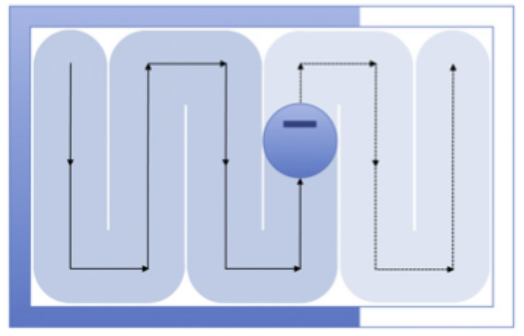
\includegraphics[width=0.4\textwidth]{figures/C3/LawnmowerPattern.png}
    \caption{Lawnmower pattern}
    \label{fig:lawnmower-pattern}
\end{figure}
\begin{figure}[ht]
    \centering
    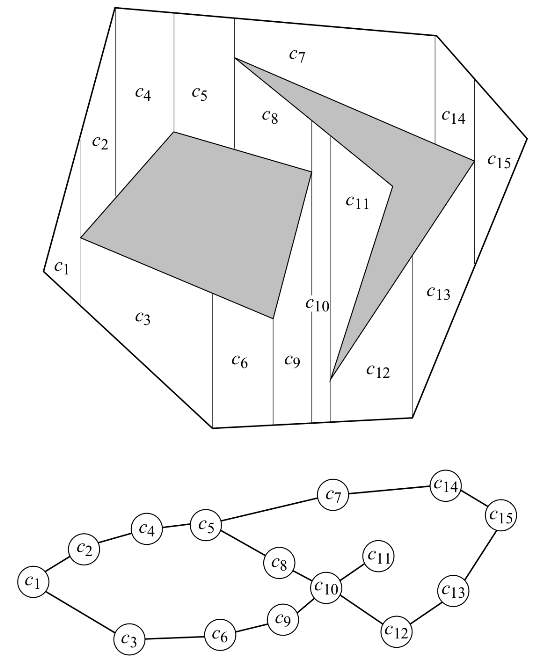
\includegraphics[width=0.4\textwidth]{figures/C3/TrapezoidalDecomposition.png}
    \caption{Trapezoidal decomposition and adjacent graph \cite{book:655068}}
    \label{fig:trapezoidal-decomposition}
\end{figure}
In trapezoidal approach many neighbor cells could be merged together into one cell resulting
in a shorter coverage path. In the left hand side of \autoref{fig:trapezoidal-boustrophedon} the robot needs to make one additional lengthwise motion to cover the remaining portion of the trapezoidal cell.
Following this idea, Choset proposed in \cite{Choset-1997-16422} an enhancement of the trapezoidal decomposition method, the \textit{Boustrophedon cellular decomposition} designed with the aim to minimize the path length by generating bigger cells.
\begin{figure}[ht]
    \centering
    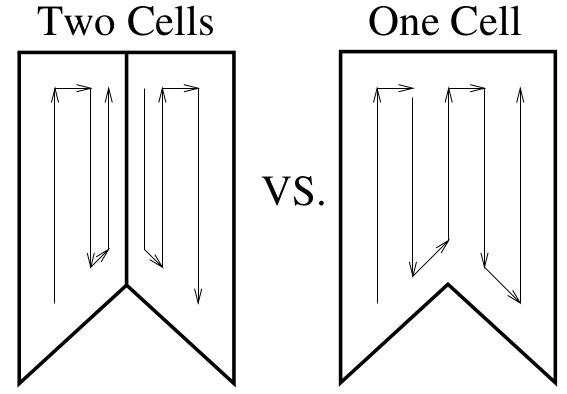
\includegraphics[width=0.3\textwidth]{figures/C3/trapezoidalVsBoustrophedon.png}
    \caption{Fewer cells is better}
    \label{fig:trapezoidal-boustrophedon}
\end{figure}
The boustrophedon decomposition is formed similarly to trapezoidal, but by considering only the vertices at which the slice can be extended both up and down in the free space (see \autoref{fig:boustrophedon-decomposition}). Such vertices are called \textit{critical points}. As before, by visiting all the nodes in the adjacency graph the area is covered completely.\par
\begin{figure}[ht]
    \centering
    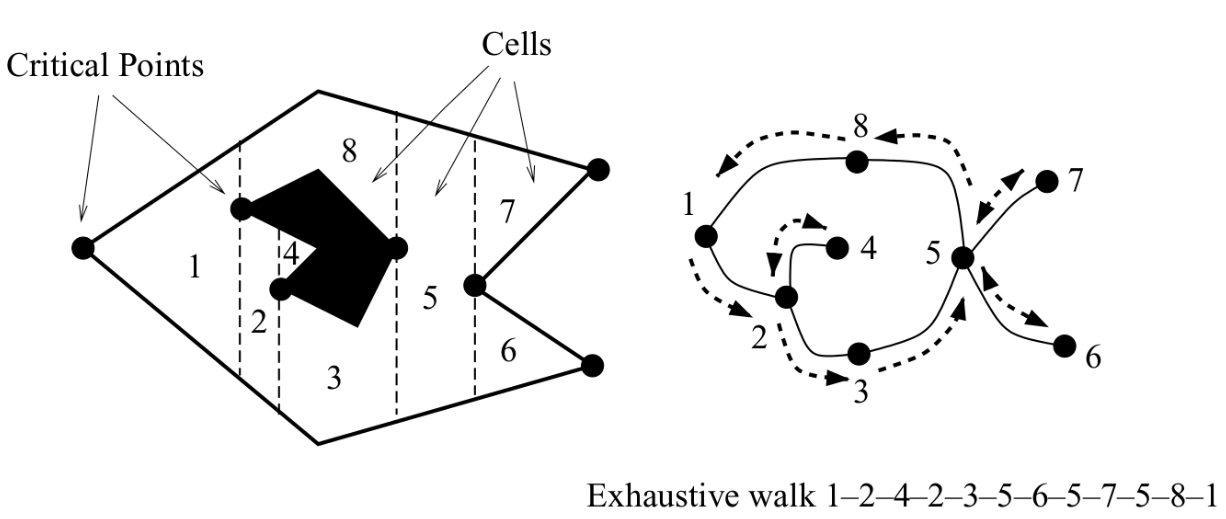
\includegraphics[width=0.65\textwidth]{figures/C3/boustrophedonDecomposition.png}
    \caption{Fewer cells is better}
    \label{fig:boustrophedon-decomposition}
\end{figure}
In summary, exact cellular decomposition guarantees a complete coverage of the target area. A bigger drawback to the trapezoidal method is that it fundamentally requires a polygonal workspace, which is not a realistic assumption for many applications. To overcome this limitation the boustrophedon decomposition was designed.
% subsubsection exact_cellular_decomposition (end)

\subsubsection{Grid-based Methods} % (fold)
\label{ssub:grid_based_methods}
Another largely used method in coverage path planning divides the environment in a collection of grid cells of the same shape. Each cell is marked as empty or occupy according to the presence of obstacle in that location. This will produce an \textit{approximate cellular decomposition} as the obstacles are represented by grid cells.
The algorithms using this grid-based representation should plan a path which visit all the empty cells of the grid minimizing the traveling cost. Primitive criteria could be to avoid revisiting cells and to move from adjacent cells only. Two interesting algorithms have been developed for this scope: The \textit{Wave-front} method \cite{Zelinsky93planningpaths} and \textit{Minimum-Spanning-Tree} (MST) method \cite{Gabriely2001}.\par
The \textit{Wave-front} method is based upon distance transform (DT) path planning methodology. This approach considered the task of path planning to finding paths from the goal location back to the start location. The path planner propagates a distance wavefront through all free space grid cells starting from the goal cell. The distance wave front flows around obstacles and eventually through all free space in the environment.\\
 \textit{"For any starting point within the environment representing the initial position of the mobile robot, the shortest path to the goal is traced by walking down hill via the steepest descent path. If there is no downhill path, and the start cell is on a plateau then it can be concluded that no path exists from the start cell to the goal cell i.e. the goal is unreachable"} \cite{Zelinsky93planningpaths}.\\
One significant advantage that distance transform path planning has over other path planning methods is that it can easily be induced to exhibit different types of robot navigation behaviors. In addition to the "optimum" i.e. shortest path behavior it is possible to have the "complete coverage" behavior. To achieve the complete coverage path planning behavior, instead of descending along the path of steepest descent to the goal, the robot follows the path of steepest ascent. In other words the robot moves away from the goal keeping track of the cells it has visited. The robot only moves into a grid cell which is closer to the goal if it has visited all the neighbouring cells which lie further away from the goal. An example of the complete coverage path is shown in \autoref{fig:wavefront}.
\begin{figure}[ht]
\centering
\begin{subfigure}{.5\textwidth}
  \centering
  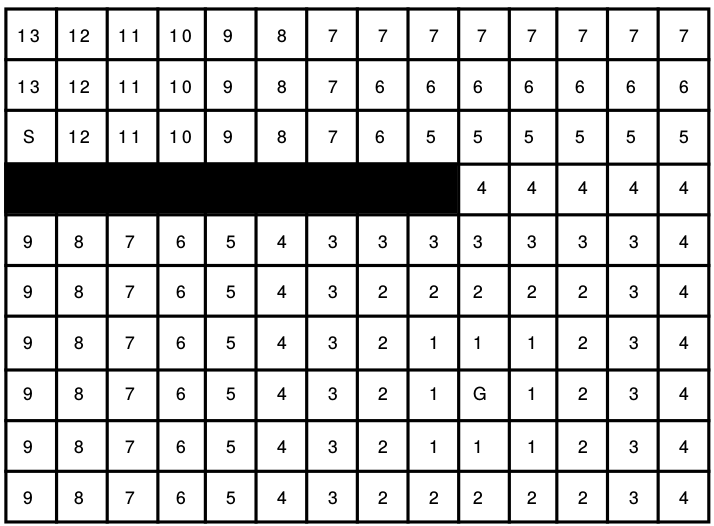
\includegraphics[width=.9\linewidth]{figures/C3/wavefrontGrid.png}
  \caption{Distance waveform grid}
\end{subfigure}%
\begin{subfigure}{.5\textwidth}
  \centering
  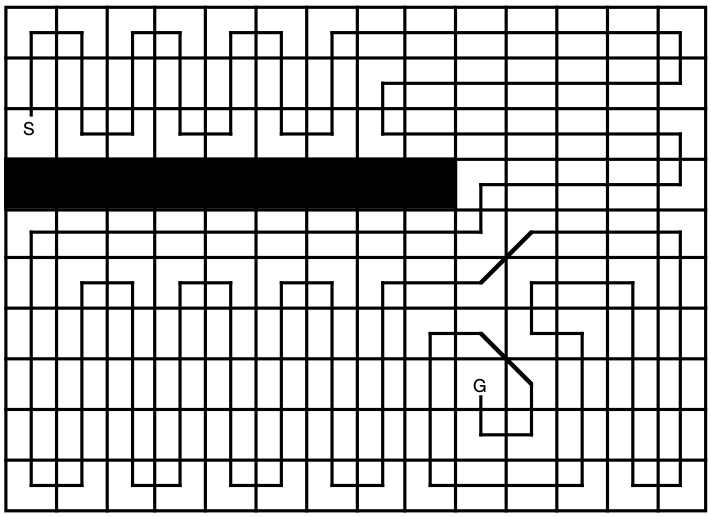
\includegraphics[width=.9\linewidth]{figures/C3/wavefrontCPath.png}
  \caption{Path of complete coverage}
\end{subfigure}
\caption{Wavefront method \cite{Zelinsky93planningpaths}}
\label{fig:wavefront}
\end{figure}
The pseudocode to obtain such behavior is listed in \autoref{alg:Wavefront-distance}.\par
A nice feature of this approach is that it is possible to set both starting and goal position. This comes in handy in cleaning or lawn mowing application. However, in some case this method can not avoid revisiting cells. Another shortcoming it is worth to highlight is the high number of turn in the coverage path. This is because the path follows the "spiral" of the distance transform wave front that radiates from the goal. A solution could be to take into account other factors than only the distance from the goal.\par
\begin{algorithm}
	\SetKwData{SCell}{startCell}\SetKwData{CCell}{currentCell}\SetKwData{Cell}{cell}\SetKwData{Stop}{stop}\SetKwData{NeighborCell}{neighborCell}
	\SetKwData{Left}{left}\SetKwData{This}{this}\SetKwData{Up}{up}
	\SetKwFunction{Union}{Union}\SetKwFunction{FindCompress}{FindCompress}
	\SetKwInOut{Input}{input}\SetKwInOut{Output}{output}

	\Input{A matrix $M$ representing the grid}
	\Output{A matrix $M$ filled with Distance Transformation}
	\BlankLine
	\SCell $\leftarrow$ \CCell \;
	\ForAll{cells of $M$}{
		 \Cell $\leftarrow$ $NotVisited$\;	
	}
	\Repeat{\Stop is true}{
		Find \textit{unvisited Neighboring cell} with highest $DT$\;
		\If(\tcc*[h]{Goal reached}){No \NeighborCell found}{
			\CCell $\leftarrow$ $Visited$\;
			\Stop $\leftarrow$ true\;
		}
		\If{\NeighborCell DT $\leq$ \CCell DT}{
			\CCell $\leftarrow$ $Visited$\;
		}
		\CCell $\leftarrow$ \NeighborCell\;
	}
\caption{CPP algorithm based on Distance Wavefront}
\label{alg:Wavefront-distance}
\end{algorithm}
The \textit{Minimum-Spanning-Tree} (MST) method only considers the cells that are completely unoccupied by obstacles [74]. First, a grid with cells 4 times the robot sensor footprint is constructed. Then a graph is created by representing each cell with a node and connecting two nodes if they are neighbor cells. The minimum spanning tree of this graph then is computed. In order to achieve complete coverage of the environment the robot circumnavigates the spanning tree visiting quadrants of the cells as shown in \autoref{fig:MST-path}. Unlike the wave-front method, this algorithm never revisits a cell and hence produces an optimal solution in terms of path length. 
\begin{figure}[ht]
    \centering
    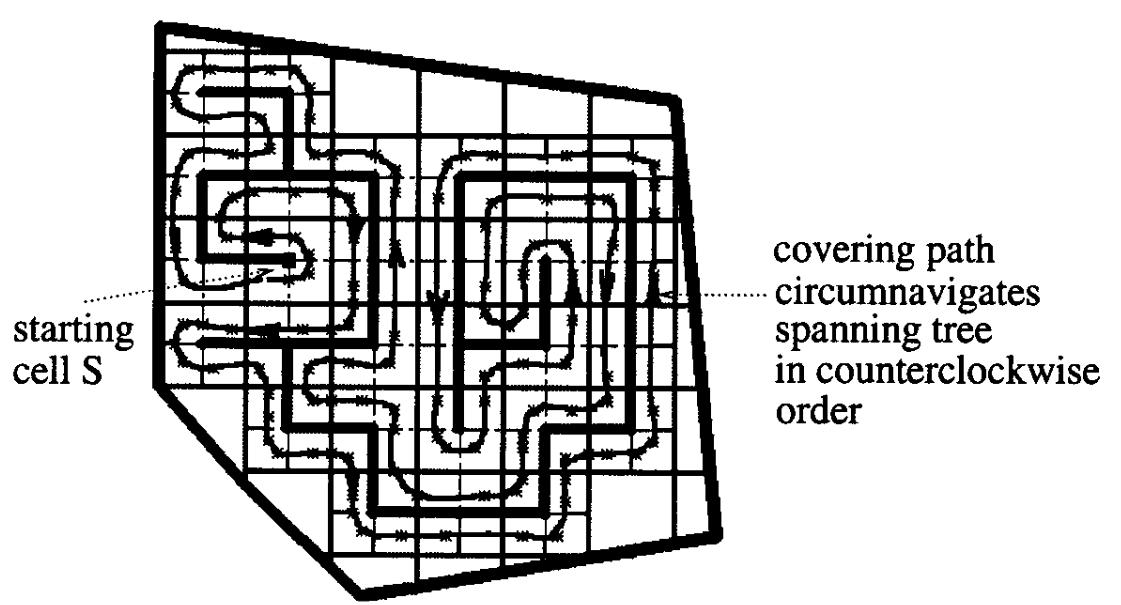
\includegraphics[width=0.65\textwidth]{figures/C3/MST-path.png}
    \caption{Minimum Spanning Tree method}
    \label{fig:MST-path}
\end{figure}
% subsubsection grid_based_methods (end)

\subsubsection{Close-loop Control methods (Online)} % (fold)
\label{ssub:close_loop_control_method}
Online approaches compute the coverage path \textit{in situ} based on sensor information, therefore unlikely offline counterpart does not require an a priori knowledge of the environment. These methods usually formulate the coverage task as an optimization problem in which the goal is to minimize (e.g., sensor overlap) or maximize (e.g., sensing of uncovered area) a metric. Howard in \cite{PotFieldCPP} developed a method in which a \textit{continuous potential field} is used to accomplish a coverage task using a team of mobile sensors. Sensors are repelled by obstacles and other team members and are consequently spread out in the area. This is a static and somehow primitive approach for CPP as it do not guarantee neither efficiency nor complete coverage, its aim is in fact to rapidly find hazards in a scenario involving hazardous materials leak in a damaged structure.\par
Other approach consist in a control law composed of two components: i) a \textit{local component} that is dependent on the coverage status of a local neighborhood, designed to direct the robot towards regions with high local coverage benefit and ii) a \textit{global component} that depends on the global coverage status and directs the robot towards a point from where the robot can cover uncovered regions \cite{6385558}.\par
A recent work by Song in \cite{8286947} present the \textit{$\varepsilon$-algorithm} (that stands for $\varepsilon$-STAR or “$\varepsilon$-coverage via structural transitions to abstract resolutions”), where $\varepsilon$ refers to the cell resolution. As shown in \autoref{fig:ETM-online-CPP}, the algorithm utilizes an Exploratory Turing Machine (ETM), that consists of a two dimensional multilevel tape formed by Multiscale Adaptive Potential Surfaces (MAPS). The ETM stores and updates the information corresponding to unexplored, explored, and obstacle-occupied regions, as time-varying potentials on MAPS. In essence, it takes advantage of both the potential field-based and sensor-based planning methods by incrementally building the MAPS using real-time sensor measurements. The ETM acts as a supervisor to the autonomous vehicle and guides it with adaptive navigation commands.
\begin{figure}[ht]
    \centering
    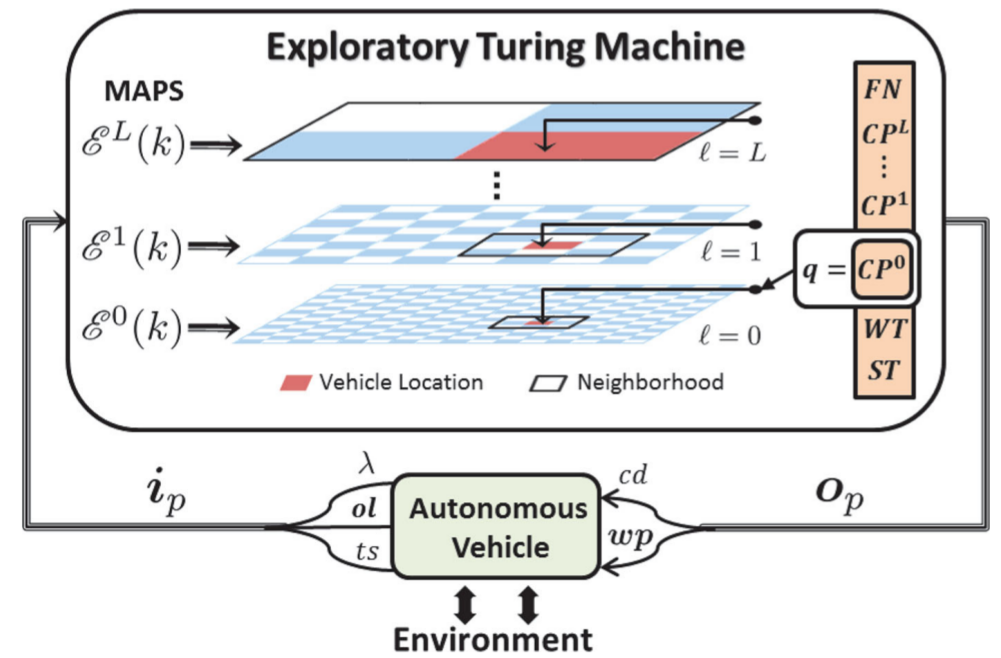
\includegraphics[width=0.65\textwidth]{figures/C3/ETM-online-CPP.png}
    \caption{ETM as a supervisor of the autonomous vehicle \cite{8286947}}
    \label{fig:ETM-online-CPP}
\end{figure}

% subsubsection close_loop_control_method (end)

% subsection coverage_path_planning_for_mobile_robots (end)
\subsection{Aerial Coverage using UAVs} % (fold)
\label{sub:aerial_coverage_using_uavs}
In aerial coverage the CPP methods presented in \autoref{sub:coverage_path_planning_for_mobile_robots} have been largely adopted (e.g. Moon \textit{et al.} in \cite{HGJHC0_2009_v10n2_1} used the Boustrophedon approach for crop dusting with multicopter). In this application the environment is specified as a grid or a polygon using GPS coordinates for polygon nodes or for the center of the cells. Obstacles are generally neglected as the flight altitude is usually high enough to avoid unwanted collision. Anyway in aerial coverage there are often uninterested regions which is out of interest in the coverage task but flight over them is allowed. For example for the specific coverage required in BambiSaver a lake is of no interest as no animals hide there. An important factor in aerial coverage using UAV is the limited flight time of the vehicle. For this reason generating an efficient path is of great importance. Along with shortening the path limiting as much as possible sensor overlap, it is relevant to minimize the number of turns in the flight trajectory. Reducing the number of turnings will produce trajectory that consist of long straight stripes. This kind of trajectory let the robot to maintain as long as possible the cruise speed, reducing acceleration and consequently power consumption.

% The general CPP methods introduced in Chapter 2.2.1 have been applied directly to aerial coverage often in an offline setting. In these works, the target area is specified as a polygon or grid with GPS coordinates of the polygon nodes or grid center. It is usually assumed that the UAV is flying at an altitude which is safe and hence there is no risk of c{}olliding with an obstacle. However sometimes some parts of the environment {}are treated as no-flying zones which should be avoided by the UAV. Therefore in CPP for UAVs, these subregions are dealt with as obstacles. Another type of region that might be present in aerial coverage is uninteresting regions. Flying in these regions is allowed but does not contribute to the coverage goal i.e. covering them is of no value. For example in a outdoor crop mapping task with a quadrotor, covering the lake is unnecessary but flying over it (for example to reach the other side of the lake) is allowed.\\
% As mentioned before, due to the very short flight time of UAVs, generating efficient coverage paths is useful. To reach efficiency, existing methods try to avoid unnecessary coverage, i.e. they try to minimize the overlap in the sensor footprint along the produced trajectory. This goal will consequently reduce the path length. Another element considered by some existing methods is to minimize the number of turns in the flight trajectory. Reducing the number of turnings will consequently produce trajectories that consist of long straight stripes, as is the case in Lawnmower pattern. Therefore, when a robot follows the trajectory it can maintain a constant velocity in a large part of the coverage path and it only accelerates or de-accelerates when it is turning. The overall outcome is less power consumption. Such efficient coverage trajectories can be planned offline when the environment is known a priori. Some of these methods, aimed for aerial coverage, are presented in the following section which includes planning for both single and multi-robot systems. However, when no prior knowledge about the target area is available, the planning has to be done online based on the real-time sensory data.\\
% In the following, we present the existing methods of coverage trajectories planning for unmanned aerial vehicles. We partition the approaches into two main groups: a) methods that precompute the trajectory based on a priori knowledge of the environment and b) methods that adaptively re-plan the trajectory based on on-line sensory data.
 % subsection aerial_coverage_using_uavs (end)

% section theory_background (end)

\section{Bambi Project CPP} % (fold)
\label{sec:proposal_solution}
The proposal implementation is based on the \textit{Wavefront} algorithm presented in \autoref{ssub:grid_based_methods}.
This algorithm has been chosen among the other for the following reasons:
\begin{itemize}
	\item The environment is known \textit{a-priori} thus an offline solution is preferable.
	\item The wavefront algorithm proved to be robust and quite efficient for aerial coverage application \cite{7496385}.
	\item This approach provide the possibility to implement different cost function, thus it is possible to obtain different behaviors (i.e. take into account of the ground elevation profile).
\end{itemize}

\subsection{Workplace Sampling} % (fold)
\label{sub:workplace_sampling}
The workplace is decomposed through approximate cellular decomposition. In this method as explained in \autoref{ssub:grid_based_methods}, the target area is divided in a grid of squared cell and a point is placed in the center of each rectangle. It has been decided to use squared shaped cells even though most of the available thermal sensor have a rectangular FOV to simplify the problem. In fact under this assumption it is possible to neglect the camera orientation and, in addition, this will produce an overlap in the recorded images which improves coverage performance compensating for the presence of small inaccuracy in the tracking of the flight trajectory. Cells dimension is chosen according to the required image resolution and it is dictated by the thermal sensor resolution. Once the cell dimension has been defined the next step is to compute the flight altitude which guarantee that the cell is completely covered by the FOV (Field of View) of the sensor when the UAV reach the point in the center of the cell. This height is maintained during the whole mission to ensure a uniform sampling of the whole field. \par

The thermal camera chosen to make the computation is the Flir Duo R a radiometric dual-sensor thermal camera specifically made for drone \cite{flir:DuoR}. The main specification of the camera are listed in \autoref{fig:FlirDuoR-specs}.\\
\begin{figure}[ht]
    \centering
    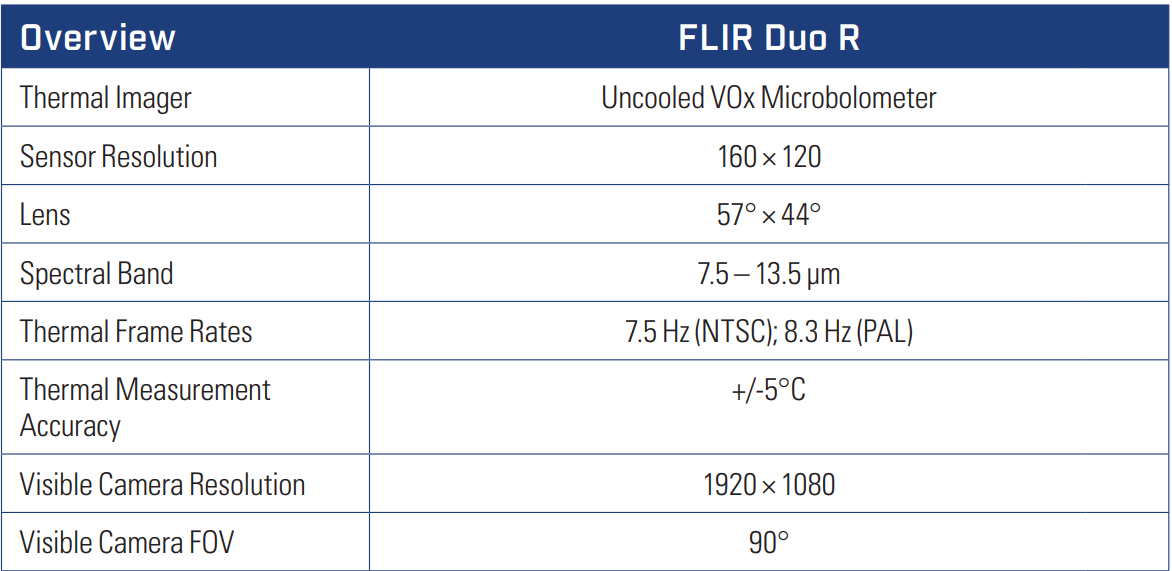
\includegraphics[width=0.65\textwidth]{figures/C3/FlirDuoR-specs.png}
    \caption{Flir Duo R thermal camera specs \cite{flir:DuoR}}
    \label{fig:FlirDuoR-specs}
\end{figure}
In the following analysis the camera is supposed to be mounted on a gimbal and facing downwards. In this way the gimbal compensate for UAV movements and keep the camera always parallel to the horizontal plane making the FOV projection easier to be computed.\\
The required FOV dimension $\tau_d$ is calculated so that one pixel of the image correspond at least to the required resolution:
\begin{gather*}
\tau_d = I_r \cdot p_{min} \\
I_r = I_t \cdot \gamma
\end{gather*}
Where:
\begin{itemize}[noitemsep]
  \item[] $I_t$: target dimension 
  \item[] $\gamma$: safe factor ($\gamma < 1$)
  \item[] $I_r$: required resolution
  \item[] $p_{min}$: minimum sensor resolution (pixels)
\end{itemize}
Each cell must be smaller then the FOV, thus: $d \leq \tau_d$. \\

The flight height $\tau_h$ is then compute from the definition of FOV:
\begin{gather*}
\tau_d = 2\,\tau_h \cdot\tan\left(\frac{\alpha}{2} \right)\\
\Rightarrow \quad \tau_h = \frac{\tau_d}{2\,\cdot\tan\left(\frac{\alpha}{2} \right)}
\end{gather*}
Where:
\begin{itemize}[noitemsep]
  \item[] $\tau_d$: FOV minimum dimension
  \item[] $\alpha$: minimum degree of the camera lens
\end{itemize}
\begin{figure}[ht]
    \centering
    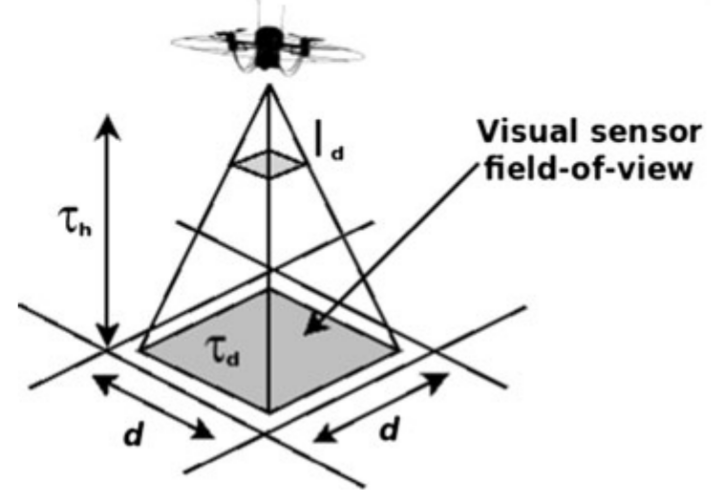
\includegraphics[width=0.6\textwidth]{figures/C3/FOV.png}
    \caption{UAV altitude and the image requirements}
    \label{fig:FOV}
\end{figure}

Now, supposing to model the target of the searching mission as a square with sides of $0.2\ cm$ (a little fawn is generally much bigger) and a safe factor $\gamma = 0.5$, then the above formulas produce the following results:
\begin{itemize}[noitemsep]
  \item[] $\tau_d = 12\,m$
  \item[] $\tau_h = 14.85\, m$
\end{itemize}
Therefore it has been decided to go for $10m \times 10m$ cells and fly at an altitude of $14\,m$ above the ground to have an adequate safe margin.
% subsection workplace_sampling (end)
\subsection{ROS Node Architecture} % (fold)
\label{sub:ros_node_architecture}
The coverage path planning algorithm is implemented in the \acrshort{ros} node named \textsf{coverage\_path\_planner}. The graph in \autoref{fig:CPP-rqt-graph} display the nodes and topics related to the CPP procedure.
\begin{figure}[ht]
    \centering
    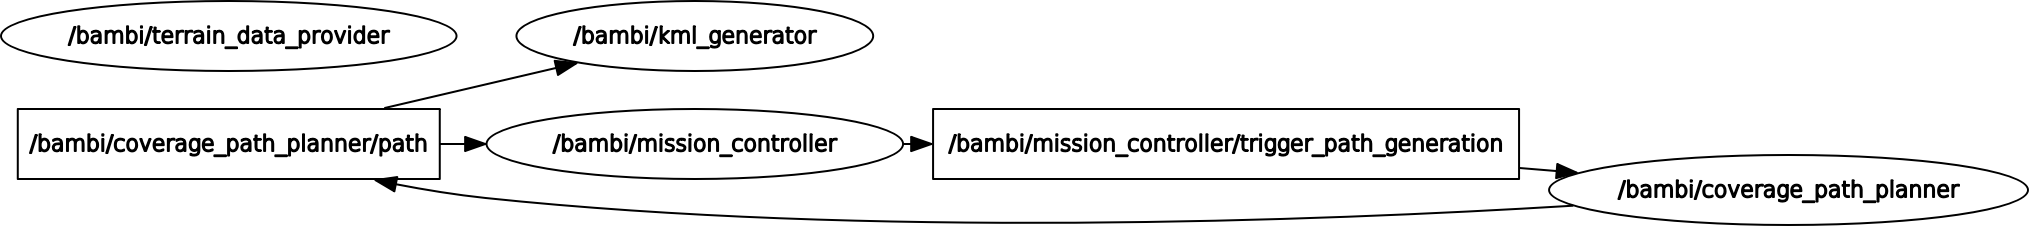
\includegraphics[width=1\textwidth]{figures/C3/CPP-rqt-graph.png}
    \caption{ROS-graph of CPP related nodes and topics}
    \label{fig:CPP-rqt-graph}
\end{figure}
The scope of the other nodes that appear in the graph are:
\begin{description}
	\item[\textsf{mission\_controller}] It handles all the mission operations as discussed in \autoref{cha:georeferencing_the_mission_s_environment}
	\item[\textsf{terrain\_data\_provider}] It provides a service (this is why in the graph it is isolated) which allow the CPP node to request terrain data. It access the Google elevation databases using Google elevation API. The inquiry is done in the form of an URL request through the python library \textsf{urllib} \cite{urllib}. 
	\item[\textsf{kml\_generator}] It generates a KML file from the CPP generated path. This task is not needed during the mission but it is of great help in debugging and for better display the CPP output.
\end{description}
The \textit{Coverage Path Planner} node task can be further divided in five sub-operations:
\begin{enumerate*}[label={(\arabic*)}]
	\item Approximate cellular Decomposition;
	\item Choosing Starting Position
	\item Wave-front Propagation Algorithm;
	\item Coverage Path Generator;
	\item Spline Interpolation.
\end{enumerate*}\par
In the following sections, first the definition of relevant \acrshort{ros} messages is given, then each sub-task is analyze separately. For parts where coding has required additional steps and consideration the implementation is analyze more in details, otherwise only the pseudocode is given for clarity and readability reasons. Anyway the whole code is accessible on the project GitHub page \cite{bambiProjectGit}.
\subsubsection{Relevant Messages Definition} % (fold)
\label{ssub:relevant_messages_definition}
Ros nodes communicate using messages over different topics. There are many build-in messages already defined in \acrshort{ros}, anyway it has been necessary to define custom messages for the specific use case. The definition of relevant messages is given in \autoref{list:msg-CPP}
\lstinputlisting[label=list:msg-CPP, caption=Relevant message definition for CPP node, language=Python]{listings/C3/relevant-ros-messages.msg}
The \textit{coverage path planner} node receives the \textsf{FieldCoverageInfo} message subscribing to the topic \textsf{/bambi/mission\_controller/trigger\_path\_generation}. The message contains the field contour data in the member type \textsf{bambi\_msg/Field} and additional information such as \textit{sensor footprint}, scanning altitude, return to home altitude, current global position and home global position. Once the path is generated the node publish a \textsf{path} message on the topic \textsf{/bambi/coverage\_path\_planner/path} 
% subsubsection relevant_messages_definition (end)

% subsection ros_node_architecture (end)
\subsection{Approximate Cellular Decomposition} % (fold)
\label{sub:approximate_cellular_decomposition}
In this section it is analyze how to decompose the workplace so that it can be represented as a grid of squared cells.\\
The cells dimension has been already computed, thus the grid dimensions are simply obtained measuring the maximum field dimensions along the horizontal and vertical axis and dividing by the cell dimension. The result of both divisions is rounded up in order to guarantee that in any case the field is smaller than the grid. The cells of the rectangular matrix so obtained, have to be marked depending on whether they are part of the field or not. The strategy adopted is to represent both the field and the cell of the grid as polygons in the same coordinates reference system. To check if a particular cell belongs to the workplace the intersection between the two polygons is performed. If the intersection exists the cell under consideration is part of the field, otherwise it is not. The \textit{approximate cellular decomposition} of the target area is so achieved. The \autoref{alg:Bambi-grid-decomposition} explain formally how to construct the grid representing the working field.
\begin{algorithm}[tbh]
	\SetKwData{x}{x}\SetKwData{l}{cellDimension}\SetKwData{LB}{leftBorderE}\SetKwData{RB}{rightBorderE}\SetKwData{BB}{bottomBorderN}\SetKwData{TB}{topBorderN}\SetKwData{w}{width}\SetKwData{h}{height}\SetKwData{nE}{nE}\SetKwData{nN}{nN}\SetKwData{Matrix}{M}\SetKwData{FieldP}{fieldPoly}\SetKwData{CellP}{cellPoly}
	\SetKwFunction{getPolygonFromMatrixCell}{getPolygonFromMatrixCell}\SetKwFunction{Ceil}{ceil}
	\SetKwInOut{Input}{input}\SetKwInOut{Output}{output}
	
	\Input{A polygon \FieldP representing the target area; The \l}
	\Output{A matrix \Matrix which correspond to the cellular decomposition of the field (i.e. where each cell is marked as "Field" or "Empty" according to whether it is part of the field or not)}
	\BlankLine
	
	\tcc{border members of the polygon object are the East or North (UTM) coordinates  of the polygon's extremities}
	\w $\leftarrow$ $\FieldP.\RB - \FieldP.\LB$ \;
	\h $\leftarrow$ $\FieldP.\TB - \FieldP.\BB$ \;

	\tcc{Computes the matrix dimensions}
	\nE $\leftarrow$ \Ceil{$\w / \l$} \;
	\nN $\leftarrow$ \Ceil{$\h / \l$} \;
	Define \Matrix as a $\nN\times\nE$-matrix\;
	\ForAll{$\x \in \Matrix$}{
			\FieldP $\leftarrow$ \getPolygonFromMatrixCell{\FieldP.\BB, \FieldP.\LB, \x, \l} \;
			\If(\tcc*[h]{cell x intersect fieldP}){$\FieldP \cap \CellP > 0$}{
				\Matrix(x) $\leftarrow$ Field\;
			}
			\Else(\tcc*[h]{cell x do not intersect fieldP}){
				\Matrix(x) $\leftarrow$ Empty\;
			}

	}
\caption{Approximate cellular decomposition of the field in a grid of squared cells}
\label{alg:Bambi-grid-decomposition}
\end{algorithm}
\subsubsection{Implementation} % (fold)
\label{ssub:implementation}
The implementation of the cellular decomposition in C++ begins with the conversion of field border geo-points from \acrshort{wgs84}\footnote{See \autoref{sec:theory_background} of \autoref{cha:georeferencing_the_mission_s_environment}} to \acrshort{utm}\footnote{\acrfull{utm} conformal projection uses a 2-dimensional Cartesian coordinate system to give locations on the surface of the Earth. The units used are meters} coordinate. This is required to obtain X (easter coordinate in \acrshort{utm}) and Y (norther coordinate in \acrshort{utm})) coordinates of each point in meters and construct the polygon representing the field.
In practice the conversion is achieved using the \textsf{geodesy} ROS package (see \cite{geodesyROS}).\par
The polygon is represented with the C++ type \textsf{boostFieldBorderPolygon} which is part of the \textsf{Boost.Geometry} library \cite{boostGeometryLib}. To define it is just required to add point-by-point the outer contour. A snapshot of the code which perform this first part of the decomposition is given in \autoref{list:cellular-decompostion-CPP}.\par
The code implementing the \autoref{alg:Bambi-grid-decomposition} is not listed because it do not add anything relevant to what already seen in the pseudocode except the specific C++ syntax and definition. An example of the output matrix is displayed in \autoref{fig:field3-decomposition-matrix} where the cells which are part of the field are marked with "XX" otherwise with "-2".
\lstinputlisting[label=list:cellular-decompostion-CPP, caption=Coordinates transformation and polygon construction in C++ , language=C++]{listings/C3/cellular-decomposition-1.cpp}
\begin{figure}[ht]
    \centering
    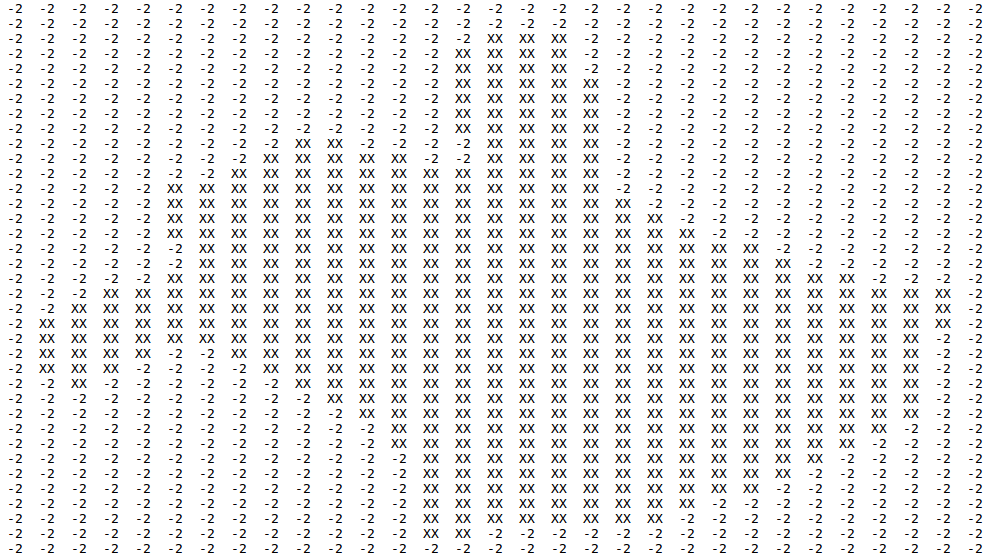
\includegraphics[width=1\textwidth]{figures/Field3/Field3-decomposition-matrix.png}
    \caption{Example of Cellular Decomposition Matrix}
    \label{fig:field3-decomposition-matrix}
\end{figure}

% subsubsection implementation (end)
% subsection approximate_cellular_decomposition (end)
\subsection{Choosing Starting Position} % (fold)
\label{sub:choosing_starting_position}
For this specific use case there is no constraint in the choice of the starting position other that it should be inside the target area. Hence it makes sense to select a smart starting position so that the path planner could generate an efficient path. After some test it seems that a good starting position is the one corresponding to the most isolated cell. Isolated in the sense that it is the cell with the lowest number of neighbors having the same cost. Among all the candidate cells, it is selected the one having the higher cost value (i.e the furthest from the goal cell).

% subsection choosing_starting_position (end)
\subsection{Wave-front Propagation Algorithm} % (fold)
\label{sub:wave_front_propagation_algorithm}
Being $G$ the grid graph, where each element represents a cell through its centroid.
Consider the navigation function: $\phi:\, G \rightarrow [1, \infty]$ which has the properties as a potential function. For the goal cell, the navigation cost $\phi(c_G)=1$ and the further the cell position to the goal cell the larger the navigation cost\footnote{In the actual implementation only distance transformation has been taken into account as cost function.}.
Once the cost has been assigned to each cell the planner algorithm will find the path which guarantees that all cells having an higher value then the goal cell are visited before the robot reaches the goal.\par

In order to construct a navigation function, we must consider the type of \textit{cell connectivity} based on the maneuverability of robot. In grid-based path planning there are two types of connectivity: the Von Neumann neighborhood (\autoref{sfig:neuman-neighborhood}) and Moore neighborhood (\autoref{sfig:moore-neighborhood}). In a Von Neumann neighborhood, the  robot turning angle is limited to $\pm 90$. In Moore neighborhood the robot will be able to turn $\pm 45$, $\pm 90$, or $\pm 135$. A quad-rotors UAV, being an \textit{holonomic} robot, it can turn at any direction rotating to any yaw angle value by changing the velocity of each motors. Therefore, it is straightforward the choice of using Moore neighborhood.
\begin{figure}[ht]
\centering
\begin{subfigure}{.3\textwidth}
  \centering
  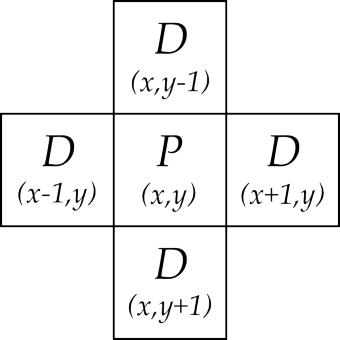
\includegraphics[width=.9\linewidth]{figures/C3/neumann-neighborhood.png}
  \caption{}
  \label{sfig:neuman-neighborhood}
\end{subfigure}
\hspace{2cm}
\begin{subfigure}{.3\textwidth}
  \centering
  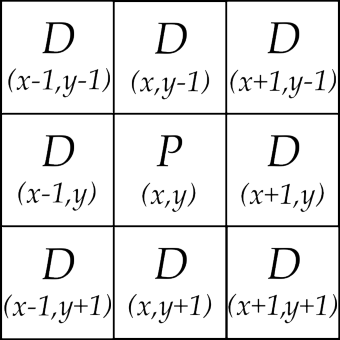
\includegraphics[width=.9\linewidth]{figures/C3/moore-neighborhood.png}
  \caption{}
  \label{sfig:moore-neighborhood}
\end{subfigure}
\caption{\ref{sfig:neuman-neighborhood} Von Neumann Neighborhood \ref{sfig:moore-neighborhood} Moore Neighborhood}
\label{fig:neighborhood}
\end{figure} 

Now using the distance transformation (as cost function) the matrix is filled starting from the goal cell. This is carried out through wave-front propagation algorithm listed in \autoref{alg:Bambi-Wavefront}.
The initial wavefront is $ W_0$, which represents the states where the current cell is the \textit{goal cell}. The algorithm can immediately assign an  optimal cost-to-go value of $ 1$ to every state that can be reached in one stage from any state in $ W_0$. The states that receive cost $ 1$ can be organized into the  wavefront $ W_1$. The unexplored neighbors of $ W_1$ are assigned cost $2$. This  process repeats inductively from $i$ to $ i+1$ until all reachable states (cells) have been reached. In the end, all the cells are filled in $O(n)$ time, in which $ n$ is the number of reachable grid states. In \autoref{fig:iwavefront-surf-f3} are represented, using 3D surface plot in Matlab, the value associated to each cell. The figure is taken from the coverage path in \autoref{sfig:F3-modified-start-goal-pos} as being the goal position in the center (the minimum point of the plot) of the field, it produce a easier to understand graph.

\begin{figure}[ht]
    \centering
    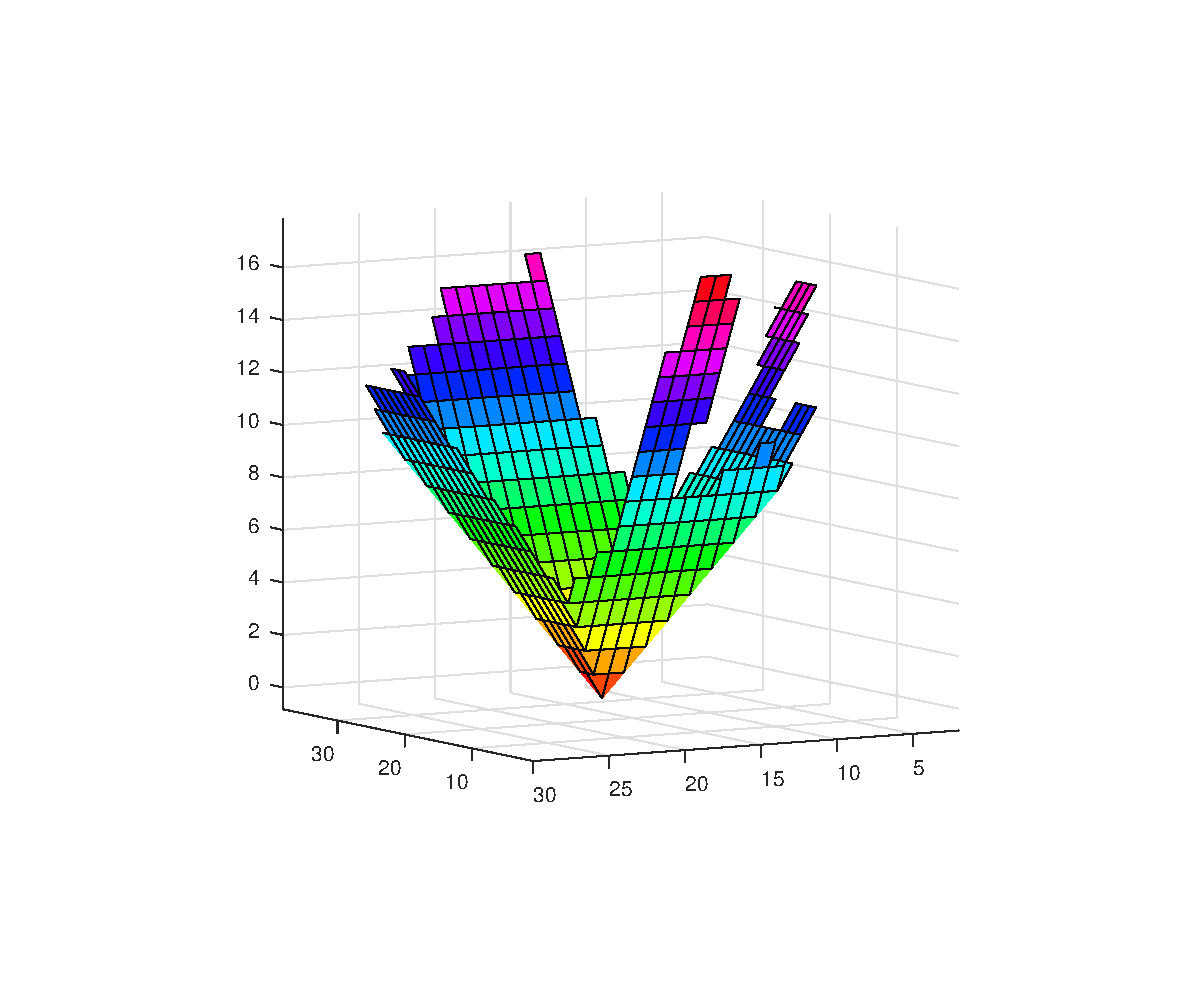
\includegraphics[width=0.95\textwidth]{figures/C3/WavefrontSurfF3-3.eps}
    \caption{Field 3 Wavefront propagation (goal position at the center)}
    \label{fig:iwavefront-surf-f3}
\end{figure}
\begin{algorithm}[H]
	\SetKwData{GCell}{goalCell}\SetKwData{x}{x}\SetKwData{W}{W}\SetKwData{Stop}{stop}\SetKwData{Matrix}{M}\SetKwData{i}{i}
	\SetKwFunction{getUnexploredNeighbors}{getUnexploredNeighbors(\Matrix, \x)}
	\SetKwInOut{Input}{input}\SetKwInOut{Output}{output}
	
	\Input{A matrix \Matrix representing the grid:;the \GCell}
	\Output{A matrix $\Matrix_o$ filled with Cost Function}
	\BlankLine
	
  	$\W_0$ $\leftarrow$ \GCell \;
	\i $\leftarrow$ 0 \;
	\Repeat{\Stop is true}{
		$\W_{i+1}$ $\leftarrow$ empty \;
		\ForAll{$\x \in \W_{\i}$}{
			$\Matrix_o$(x) $\leftarrow$ \i \;	
			$\W_{i+1}$ $\leftarrow$ \getUnexploredNeighbors \;
		}
		\i $\leftarrow$ \i+1 \;
		\If(\tcc*[h]{No more cells to expand}){$\W_{i+1}$ is empty}{
			\Stop $\leftarrow$ true\;
		}
	}
\caption{Filling matrix using Wavefront propagation starting from the \textit{goal} cell}
\label{alg:Bambi-Wavefront}
\end{algorithm}


% subsection wave_front_propagation_algorithm (end)

\subsection{Coverage Path Generator} % (fold)
\label{sub:coverage_path_generator}
Once the elements matrix has been filled according to the cost function, the last step is to generate the path which assure that each cell is visited. This is done through a gradient ascending searching algorithm from the start cell. All the unvisited neighbors of the current cell are evaluated and for each is given a \textit{priority}. The neighbor having the higher priority is appointed and selected as the current cell for the next step of the iteration. The process continues until there are no more unvisited neighbors.\par
\textit{Priority} function takes into account different features of the neighbors cells which are in order of relevance:
\begin{enumerate}
	\item The cost function value associated to that cell
	\item How many adjacent cells have the same value, favoring the neighbor which has the lower number of same value adjacent cells. This is to avoid as much as possible the risk of reaching a local minimum which could cause the algorithm to stack.
	\item The Von Neumann neighbors are preferred, i.e the diagonal neighbors have less priority because they are a little farther ($\sqrt{2}\,l$ instead of just $l$ as it is for Von Neumann neighbors)
\end{enumerate}
The pseudocode which plan the coverage path is listed in \autoref{alg:Bambi-pathPlanner}.\\
\begin{algorithm}[H]
	\SetKwData{SCell}{startCell}\SetKwData{CCell}{currentCell}\SetKwData{x}{x}\SetKwData{W}{W}\SetKwData{Stop}{stop}\SetKwData{Matrix}{M}\SetKwData{P}{P}\SetKwData{reachedEnd}{reachedEnd}\SetKwData{bestPriority}{bestPriority}\SetKwData{N}{N}\SetKwData{priority}{priority}\SetKwData{bestChoice}{bestChoice}
	\SetKwFunction{getUncoveredNeighbors}{getUncoveredNeighbors}\SetKwFunction{isDiagonalCell}{isDiagonalCell}\SetKwFunction{nSameValuedNeighbors}{nSameValuedNeighbors}\SetKwFunction{getCentroidCoordinates}{getCentroidCoordinates}\SetKwFunction{pushBack}{push\_back}
	\SetKwInOut{Input}{input}\SetKwInOut{Output}{output}
	
	\Input{the grid matrix \Matrix filled with Distance Transformation values; the \SCell}
	\Output{A vector \P of waypoints representing the coverage path}
	\BlankLine
	\
  	\CCell $\leftarrow$ \SCell \;
	\reachedEnd $\leftarrow$ false \;
	\While{not \reachedEnd}{
		\reachedEnd $\leftarrow$ true \;
		\bestPriority $\leftarrow$ -1 \;
		\N $\leftarrow$ \getUncoveredNeighbors{\Matrix, \CCell} \;
		\ForAll{$\x \in \N$}{
			\reachedEnd $\leftarrow$ false \;
			\priority $\leftarrow$ $\Matrix{\CCell}*100+ (8-\nSameValuedNeighbors{\Matrix, \x}*10 + 1$\;
			\If(\tcc*[h]{It is a diagonal cell}){\isDiagonalCell{\CCell, \x}}{
				\priority $\leftarrow$ $\priority - 1$ \;
			}
			\If(\tcc*[h]{find highest priority cells}){$\priority > \bestPriority$}{
				\bestPriority $\leftarrow$ \priority \;
				\bestChoice $\leftarrow$ \x \;
			}
		}
		\If{not \reachedEnd}{
			\Matrix{\CCell} $\leftarrow$ Covered\;
			\P.\pushBack{\getCentroidCoordinates{\CCell}} \;
			\CCell $\leftarrow$ \bestChoice \;
		}
	}
\caption{Generating Coverage Path}
\label{alg:Bambi-pathPlanner}
\end{algorithm}

% subsection coverage_path_generator (end)
\subsection{Spline Interpolation} % (fold)
\label{sub:spline_interpolation}
The resulting coverage path is a piecewise function in the local reference system made up of segment connecting the center of the cells in the order provided by the algorithm shown in \autoref{sub:coverage_path_generator}. Therefore the outcome path is really sharply and edgy. Before sending the trajectory to the vehicle it is then required to smooth it. This is done using spline interpolation. Spline interpolation is a form of interpolation where the interpolant is a special type of piecewise polynomial called a spline. This subject goes outside the  scope of the thesis, thus only the implementation is given.


\subsubsection{Implementation} % (fold)
\label{ssub:implementation}
The implementation in C++ relay on the \textit{cpp-spline} Library provided by Xianshun Chen who make it available on GitHub \cite{cpp-spline}. \autoref{fig:CPP-matlab} shows the path before and after the interpolation. The smoothing effect is evident since the algorithm produce a piecewise function imposing continuity up to second order derivative. This positive features comes at the expenses of accuracy, because the resulting spline does not exactly pass through every given point as evidenced in \autoref{fig:interpolation-error}. Fortunately this inaccuracy has a little impact on coverage performance due to sensor overlap considered in the computation of the flight altitude (see \autoref{sub:workplace_sampling}).
\begin{figure}[H]
\centering
\begin{subfigure}{.49\textwidth}
  \centering
  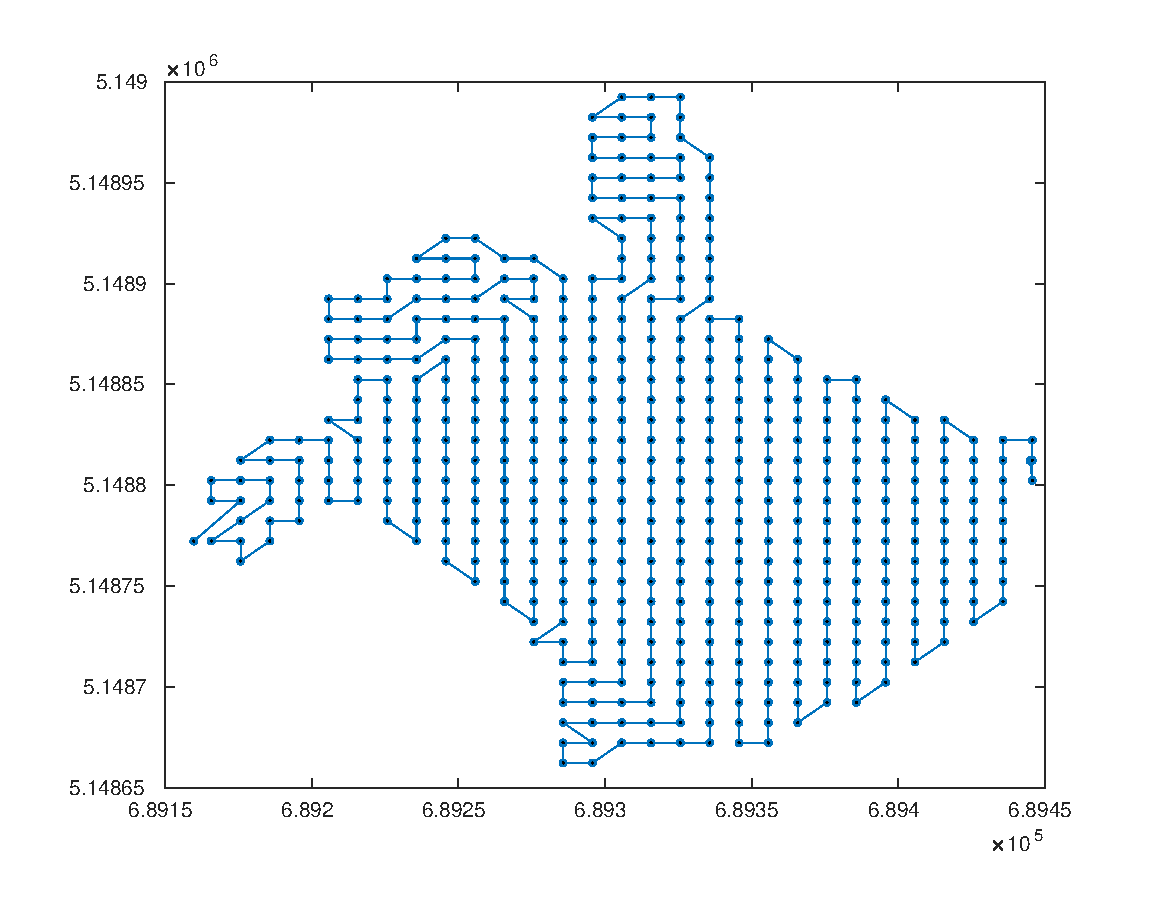
\includegraphics[width=.99\linewidth]{figures/C3/CPP-path-marker.eps}
  \caption{}
  \label{sfig:CPP-path-matlab}
\end{subfigure}
\begin{subfigure}{.49\textwidth}
  \centering
  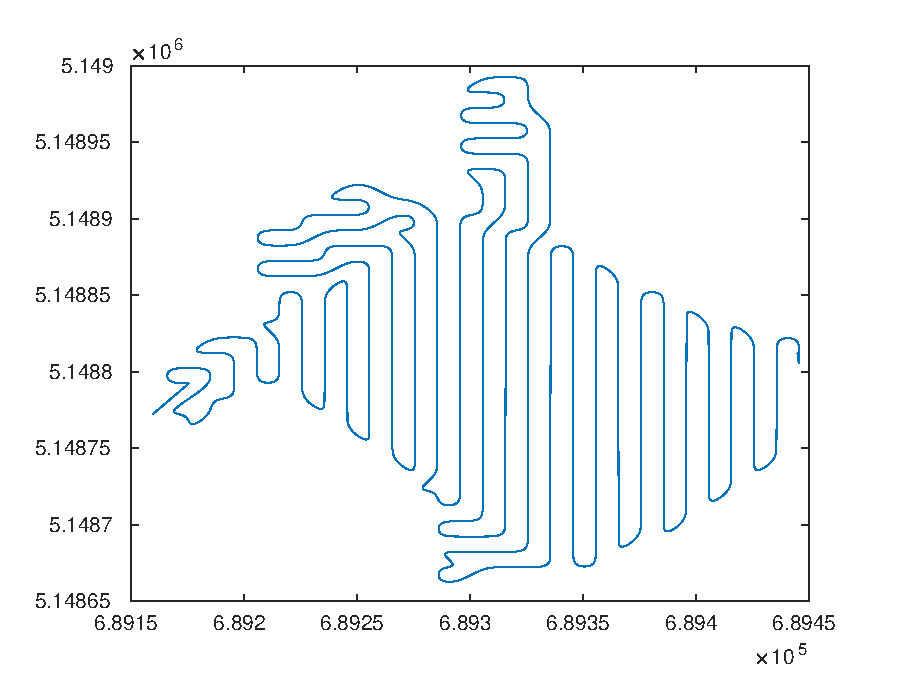
\includegraphics[width=.99\linewidth]{figures/C3/CPP-path-spline.eps}
  \caption{}
  \label{sfig:CPP-path-spline-matlab}
\end{subfigure}
\caption{CPP path (\subref{sfig:CPP-path-matlab})before and (\subref{sfig:CPP-path-spline-matlab})after interpolation}
\label{fig:CPP-matlab}
\end{figure}
\begin{figure}[H]
    \centering
    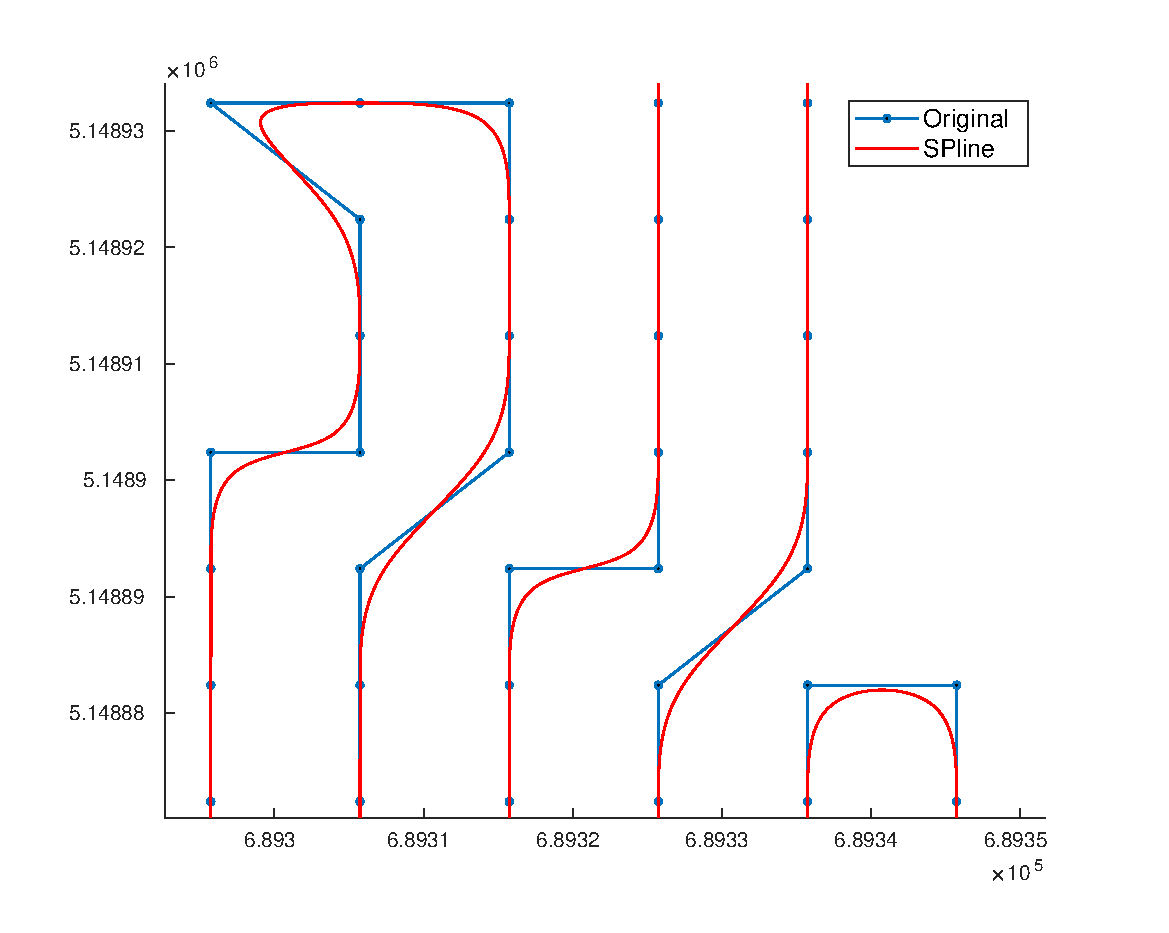
\includegraphics[width=0.39\textwidth]{figures/C3/Interpolation-error.eps}
    \caption{Interpolation error}
    \label{fig:interpolation-error}
\end{figure}



% subsubsection implementation (end)
% subsection spline_interpolation (end)



% !!!!!!Da mettere nella scelta della starting position !!!!!!!
% The starting position is chosen as the cell having the higher 


% section cpp_algorithms (end)